% article example for classicthesis.sty
\documentclass[10pt,a4paper]{article} % KOMA-Script article scrartcl
\usepackage{import}
\usepackage{xifthen}
\usepackage{pdfpages}
\usepackage{transparent}
\newcommand{\incfig}[1]{%
    \def\svgwidth{\columnwidth}
    \import{./figures/}{#1.pdf_tex}
}
\usepackage{lipsum}     %lorem ipsum text
\usepackage{titlesec}   %Section settings
\usepackage{titling}    %Title settings
\usepackage[margin=10em]{geometry}  %Adjusting margins
\usepackage{setspace}
\usepackage{listings}
\usepackage{amsmath}    %Display equations options
\usepackage{amssymb}    %More symbols
\usepackage{xcolor}     %Color settings
\usepackage{pagecolor}
\usepackage{mdframed}
\usepackage[spanish]{babel}
\usepackage[utf8]{inputenc}
\usepackage{longtable}
\usepackage{multicol}
\usepackage{graphicx}
\graphicspath{ {./Images/} }
\setlength{\columnsep}{1cm}

% ====| color de la pagina y del fondo |==== %
\pagecolor{black}
\color{white}



\begin{document}
    %========================{TITLE}====================%
    \title{\rmfamily\normalfont\spacedallcaps{ Tarea 1 de Teoría de grafos }}
    \author{\spacedlowsmallcaps{Rodrigo Castillo}}
    \date{\today}

    \maketitle

    %=======================NOTES GOES HERE===================%
    \section{calcule el complemento de los siguientes grafos}
        \subsection{grafo G}
            complmento grafo $ G  $
            \\
            \begin{figure}[h]
                \centering
                \incfig{primerpunto}
                \caption{primerpunto}
                \label{fig:grafo G}
            \end{figure}
        \subsection{Grafo H}
            complemento grafo $ H  $
            \\
            \begin{figure}[h]
                \centering
                \incfig{grafoh}
                \caption{grafoH}
                \label{fig:grafo H}
            \end{figure}
    \section{adicionalmente escriba la matriz de adyascencia de G y la matriz de incidencia de H}
        \subsection{matriz de adyascencia de G}
        se tiene el grafo $ [a-b,a-e , e-b ,e-d ,d-b , b-c]  $
        cuya matriz se escribo como :
        \begin{equation}
            M_G = \begin{pmatrix}
                 0 & 1 & 0 & 0 & 1
                \\1 & 0 & 1 & 1 & 1
                \\0 & 1 & 0 & 0 & 0
                \\0 & 1 & 0 & 0 & 0
                \\1 & 1 & 0 & 0 & 0
            \end{pmatrix}
        \end{equation}
        \subsection{Matriz de incidencia de h}
            se tiene el grafo H, luego su matriz de incidencia se expresa como :
            \begin{equation}
                M_H = \begin{pmatrix}
                    1 & 1 & 1 & 0 & 0 & 0 & 0 & 0
                    \\ 0 & 0 & 1 & 0 & 1 & 0 & 0 & 1
                    \\ 1 & 0 & 0 & 1 & 0 & 1 & 0 & 0
                    \\ 0 & 0 & 0 & 0 & 0 & 1 & 1 & 1
                    \\ 0 & 1 & 1 & 1 & 0 & 0 & 1 & 0
                \end{pmatrix}
            \end{equation}
    \section{Encuentre un conjunto independiente de tamaño maximo
    en el grafo G y un clique de tamaño maximo en el grafo H}
        \subsection{Conjunto independiente en G}
        $ [b,c,d]  $
        \subsection{clique en H}
        $ [a,b,c,d,e]  $

    \section{Escriba la matriz de adyascencia e incidencia del siguiente grafo}
        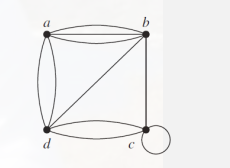
\includegraphics[width=0.5\linewidth]{grafo.png}
        \\
        \subsection{Matriz de adyascencia}
            \begin{equation}
                M_a = \begin{pmatrix}
                    0 & 3 & 0 & 2
                  \\3 & 0 & 1 & 1
                  \\0 & 1 & 1 & 2
                  \\2 & 1 & 2 & 0
                \end{pmatrix}
            \end{equation}
        \subsection{Matriz de incidencia}
            \begin{equation}
                M_i = \begin{pmatrix}
                     1 & 1 & 1 & 1 & 1 & 0 & 0 & 0 & 0 & 0
                    \\1 & 1 & 1 & 0 & 0 & 1 & 1 & 0 & 0 & 0
                    \\0 & 0 & 0 & 1 & 1 & 1 & 1 & 1 & 0 & 0
                    \\0 & 0 & 0 & 0 & 0 & 0 & 1 & 1 & 1 & 1
                \end{pmatrix}
            \end{equation}
    \section{Dibuje los grafos correspondientes a las siguientes matrices}
        \subsection{primer grafo}
            primer dibujo:
            \\
            \begin{figure}[h]
                \centering
                \incfig{primerdibujo}
                \caption{primerdibujo}
                \label{fig:grafo de la matriz}
            \end{figure}
    \section{Escriba la forma general de la matriz de incidencia de un grafo $ K_n  $ }
        la matriz de adyacencia de un grafo $ K_n  $ es de la forma:
        \begin{equation}
            M_{kn} = \begin{pmatrix}
                0 & 1 & 1 & ... & 1
                \\ 1 & 0 & 1 & ... & 1
                \\ & & . & &
                \\ & & . & &
                \\ & & . & &
                \\1 & 1 & 1 & ... & 0
            \end{pmatrix}
        \end{equation}
        donde el de la matrix $ M_{ij}  $ en el cuál $ i=j  $ es igual a 0 y
        el resto de los elementos de la matriz son iguales a 1























    %=======================NOTES ENDS HERE===================%

    % bib stuff
    \nocite{*}
    \addtocontents{toc}{\protect\vspace{\beforebibskip}}
    \addcontentsline{toc}{section}{\refname}
    \bibliographystyle{plain}
    \bibliography{../Bibliography}
\end{document}
